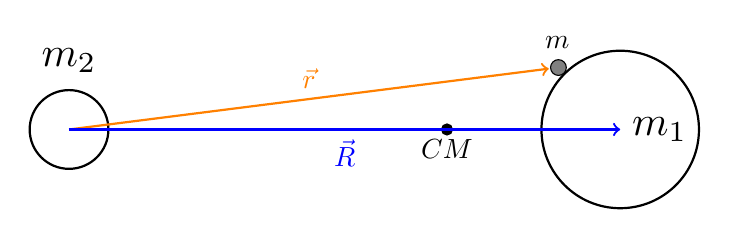
\begin{tikzpicture}
\draw [thick,] (1.5,0.5) node (v1) {} circle (1);
\draw [thick] (-5.5,0.5) circle (0.5)node [scale=1.5, above =10]{$m_2$};
\draw [->, thick, orange](-5.5,0.5) -- (0.5926,1.2722)node [midway, above]{$\vec{r}$};
\draw  [fill](-0.7,0.5) circle (0.07) node [below]{$CM$};
\node at (0.7,1.6) {$m$};
\draw [->,blue, thick](-5.5,0.5) -- (1.5,0.5) node [midway, below]{$\vec{R}$};
\node [scale=1.5] at (2,0.5) {$m_1$};
\draw  [fill=gray](0.7154,1.2866) circle (0.1);
\end{tikzpicture}